\documentclass[english,handout,10pt,aspectratio=169,t]{beamer}

\usepackage{amsmath}
\usepackage{array}
\usepackage[T1]{fontenc}
\usepackage{listings}
\usepackage{tikz}
\usepackage{ulem}

%%%%%%%%%%%%%%%%%%%%%%%%%%%%%%%%%%%%%%%%%%%%%%%%%%%%%%%%%%%
% beamer
%%%%%%%%%%%%%%%%%%%%%%%%%%%%%%%%%%%%%%%%%%%%%%%%%%%%%%%%%%%
\mode<presentation>
\usetheme{singapore}
\usecolortheme{orchid}

%%%%%%%%%%%%%%%%%%%%%%%%%%%%%%%%%%%%%%%%%%%%%%%%%%%%%%%%%%%
% listings
%%%%%%%%%%%%%%%%%%%%%%%%%%%%%%%%%%%%%%%%%%%%%%%%%%%%%%%%%%%
\lstdefinestyle{PythonStyle}{
	basicstyle=\scriptsize\ttfamily,
	language=Python,
	numbers=left,
	tabsize=4
}
\lstset{basicstyle=\small,style=PythonStyle}

%%%%%%%%%%%%%%%%%%%%%%%%%%%%%%%%%%%%%%%%%%%%%%%%%%%%%%%%%%%
% tikz
%%%%%%%%%%%%%%%%%%%%%%%%%%%%%%%%%%%%%%%%%%%%%%%%%%%%%%%%%%%
\usetikzlibrary{shapes.geometric, arrows}
\tikzstyle{startstop} = [
	rectangle,
	rounded corners,
	minimum width=1cm,
	minimum height=0.5cm,
	text centered,
	draw=black,
	fill=red!30
]
\tikzstyle{io} = [
	trapezium,
	trapezium left angle=70,
	trapezium right angle=110,
	minimum width=1cm,
	minimum height=0.5cm,
	text centered,
	draw=black,
	fill=blue!30
]
\tikzstyle{process} = [
	rectangle,
	minimum width=1cm,
	minimum height=0.5cm,
	text centered,
	draw=black,
	fill=orange!30
]
\tikzstyle{decision} = [
	diamond,
	minimum width=1cm,
	minimum height=0.5cm,
	text centered,
	draw=black,
	fill=green!30
]
\tikzstyle{arrow} = [thick, ->, >=stealth]
%%%%%%%%%%%%%%%%%%%%%%%%%%%%%%%%%%%%%%%%%%%%%%%%%%%%%%%%%%%
% commands
%%%%%%%%%%%%%%%%%%%%%%%%%%%%%%%%%%%%%%%%%%%%%%%%%%%%%%%%%%%
\newcommand{\focus}[1]{\textcolor{blue}{#1}}

\newcommand{\hideit}[1]{%
  \only<0| handout:1>{\mbox{}}%
  \invisible<0| handout:1>{#1}%
}

\def\presentationtitle{\textbf{
  Spending less time bug fixing by \\
  spending more time unit testing
}}

\title{\large\presentationtitle}
\author{\textbf{
  <Name>
}}
\date{}

\begin{document}

%%%%%%%%%%%%%%%%%%%%%%%%%%%%%%%%%%%%%%%%%%%%%%%%%%%%%%%%%%%
% code listings 
%%%%%%%%%%%%%%%%%%%%%%%%%%%%%%%%%%%%%%%%%%%%%%%%%%%%%%%%%%%
\defverbatim[colored]\coveragecode{%
\begin{lstlisting}[linewidth=0.5\textwidth]
def is_fizzbuzz(num: int) -> bool:
    if num % 3 and num % 5:
        return True
    return some_var

def test_fizzbuzz():
    result = is_fizzbuzz(3)
    assert result
\end{lstlisting}
}

\defverbatim[colored]\coveragecodetwo{%
\begin{lstlisting}[linewidth=0.5\textwidth]
def is_fizzbuzz(num: int) -> bool:
    return True if num % 3 and num % 5 else some_var

def test_fizzbuzz():
    result = is_fizzbuzz(3)
    assert result
\end{lstlisting}
}

\defverbatim[colored]\coveragecodebranch{%
\begin{lstlisting}[linewidth=0.5\textwidth]
def generate_number(
    cond_1: bool = True,
    cond_2: bool = True,
    cond_3: bool = True,
) -> int:
    if cond_1:
        num = 1
    if cond_2:
        num = 2
    if cond_3:
        num = 3
    return num
\end{lstlisting}
}


\begin{frame}
  \titlepage
\end{frame}

% To begin with a quote from the author, "There's much more to unit testing than
% the act of writing tests." Hopefully this presentation will be able to get you
% to think more about how to craft unit tests.
\begin{frame}
  \vfill
  \begin{quote}
    There's much more to unit testing than the act of writing tests.
    \begin{flushright}
      \tiny{---Khorikov, \textup{Unit Testing Principles, Practices, and Patterns}, 3}
    \end{flushright}
  \end{quote}
  \vfill
\end{frame}

% The goal of unit testing is to enable sustainable growth of the software
% project. The figure below show the growth dynamics of a typical project without
% tests. You start off quick, completing user stories after user stories, without
% having to "waste" writing these pesky tests.
% But eventually progress slows to a halt, the code base has grown complex and
% disorganized, fixing one bug introduces several others, and changing one part
% of the software breaks several others. And it's hard to bring it back to
% stability.
% This is where tests help, they help detect regressions and ensure existing
% functionalities work even after refactoring or introducing new features.
\begin{frame}{The goal of unit testing}
  To enable \textbf{sustainable} growth of software project.
  \begin{columns}[T]
    \begin{column}{0.5\textwidth}
      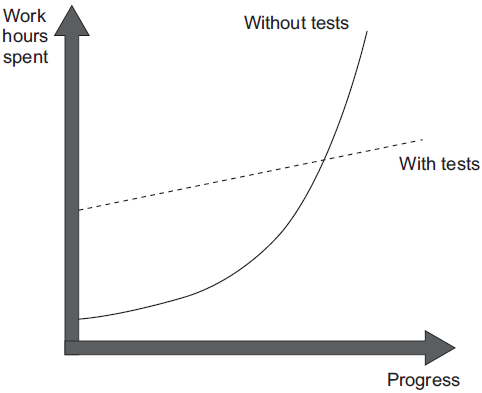
\includegraphics[width=\textwidth]{images/vs_no_test.png}
    \end{column}
    \begin{column}{0.5\textwidth}
    \end{column}
  \end{columns}
\end{frame}

% But it's not enough to just write tests. Badly written tests still result in
% the same picture. They help slow down the initial decline in development speed
% but doesn't really change much overall. Before we look at what makes a good unit
% test, let's first look at code coverage metrics which can help you gauge if you
% are testing enough.
\begin{frame}{The goal of unit testing}
  To enable \textbf{sustainable} growth of software project.
  \begin{columns}[T]
    \begin{column}{0.5\textwidth}
      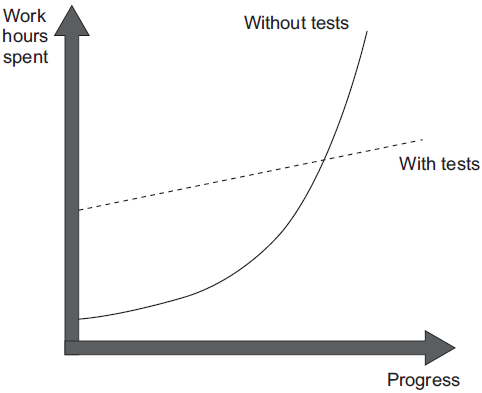
\includegraphics[width=\textwidth]{images/vs_no_test.png}
    \end{column}
    \begin{column}{0.5\textwidth}
      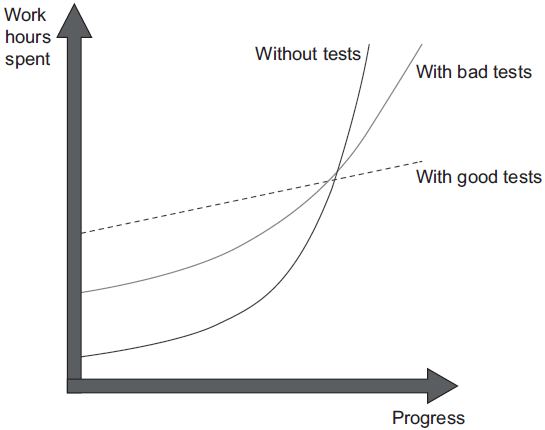
\includegraphics[width=\textwidth]{images/vs_bad_test.png}
    \end{column}
  \end{columns}
\end{frame}

% The common belief is that the higher the coverage number, the better the test
% suite. Unfortunately, it's not that simple. While 10% is a good indication
% that you aren't testing enough, 100% coverage doesn't guarantee you have a
% good quality test suite. We take a look at a few coverage metrics to see why
% this is so.
% We will discuss 4 types of coverage metrics. Path and condition coverage are
% struck out because while they're nice to think about, they're impractical to
% actually implement.
% < describe the code and coverage stats > 
\begin{frame}{Coverage metrics}
  \focus{Statement} vs Branch vs \sout{Path} vs \sout{Condition}
  \begin{columns}[T]
    \begin{column}[]{0.6\textwidth}
      \begin{minipage}{\linewidth}
        \coveragecode
      \end{minipage}
    \end{column}
    \begin{column}[]{0.4\textwidth}
      \begin{flalign*}
        &\frac{Number\ of\ statements\ executed}{Total\ number\ of\ statements}\\
        \approx\ &67 \%
      \end{flalign*}
    \end{column}
  \end{columns}
\end{frame}

% One simple trick to improve our statement coverage metric to refactor the
% function into a conditional expression. Now we get 100% statement coverage
% without having to write any extra tests. This just shows how easy it is to game
% the coverage metrics.
\begin{frame}{Coverage metrics}
  \focus{Statement} vs Branch vs \sout{Path} vs \sout{Condition}
  \begin{columns}[T]
    \begin{column}[]{0.6\textwidth}
      \begin{minipage}{\linewidth}
        \coveragecodetwo
      \end{minipage}
    \end{column}
    \begin{column}[]{0.4\textwidth}
      \begin{flalign*}
        &\frac{Number\ of\ statements\ executed}{Total\ number\ of\ statements}\\
        =\ &100 \%
      \end{flalign*}
    \end{column}
  \end{columns}
\end{frame}

% Branch coverage considers how many control structures are traversed by at least
% one test in the test suite. And reports 50% coverage no matter how we refactor
% the function.
\begin{frame}{Coverage metrics}
  Statement vs \focus{Branch} vs \sout{Path} vs \sout{Condition}
  \begin{columns}[T]
    \begin{column}[]{0.6\textwidth}
      \begin{minipage}{\linewidth}
        \coveragecodetwo
      \end{minipage}
    \end{column}
    \begin{column}[]{0.4\textwidth}
      \begin{flalign*}
        &\frac{Branches\ traversed}{Total\ number\ of\ branches}\\
        =\ &50 \%
      \end{flalign*}
    \end{column}
  \end{columns}
\end{frame}

% To help visualize this metric, the flowchart shows the possible paths of the
% function. And the test_fizzbuzz() function only traversed through one of them.
\begin{frame}{Coverage metrics}
  Statement vs \focus{Branch} vs \sout{Path} vs \sout{Condition}
  \begin{columns}[T]
    \begin{column}[]{0.6\textwidth}
      \begin{minipage}{\linewidth}
        \coveragecodetwo
      \end{minipage}
    \end{column}
    \begin{column}[]{0.4\textwidth}
      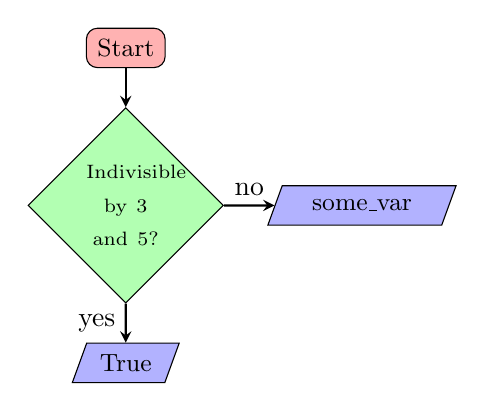
\begin{tikzpicture}[node distance=2cm]
        \node (start) [startstop] {\small{Start}};
        \node (decision)
          [decision, below of=start, text width=1cm, align=center]
          {\scriptsize{Indivisible by 3 and 5?}};
        \node (out1) [io, below of=decision] {\small{True}};
        \node (out2) [io, right of=decision, xshift=1cm] {\small{some\_var}};
        \draw [arrow] (start) -- (decision);
        \draw [arrow] (decision) -- node[anchor=east] {yes} (out1);
        \draw [arrow] (decision) -- node[anchor=south] {no} (out2);
      \end{tikzpicture}
    \end{column}
  \end{columns}
\end{frame}

% This function has 3 if conditions each returning a different number. Branch
% coverage requires 6 test cases. But does achieving 100% branch coverage
% ensure that this function won't crash? What happens when all 3 conditions
% evaluate to False? Path coverage ensures all paths are covered. It will test
% path BDF and catch the bug. Although this will give you a very comprehensive
% coverage of your code, 100% path coverage is impractical to aim for in reality.
\begin{frame}{Coverage metrics}
  Statement vs Branch vs \focus{\sout{Path}} vs \sout{Condition}
  \begin{columns}[T]
    \begin{column}[]{0.5\textwidth}
      \begin{minipage}{\linewidth}
        \coveragecodebranch
        Possible paths:

        ACE, ACF, ADE, ADF, BCE, BCF, BDE, BDF
      \end{minipage}
    \end{column}
    \begin{column}[]{0.5\textwidth}
      \begin{tikzpicture}[node distance=1.3cm]
        \node (start) [startstop] {\small{Start}};
        \node (dec1) [decision, below of=start, aspect=3, yshift=1mm]
          {\scriptsize{cond\_1?}};
        \node (out11) [io, left of=dec1, xshift=-1.75cm, label={A}]
          {\small{num = 1}};
        \node (out12) [io, right of=dec1, xshift=1cm, label={B}] {\small{pass}};
        \node (dec2) [decision, below of=dec1, aspect=3]
          {\scriptsize{cond\_2?}};
        \node (out21) [io, left of=dec2, xshift=-1.75cm, label={C}]
          {\small{num = 2}};
        \node (out22) [io, right of=dec2, xshift=1cm, label={D}] {\small{pass}};
        \node (dec3) [decision, below of=dec2, aspect=3]
          {\scriptsize{cond\_3?}};
        \node (out31) [io, left of=dec3, xshift=-1.75cm, label={E}]
          {\small{num = 3}};
        \node (out32) [io, right of=dec3, xshift=1cm, label={F}] {\small{pass}};
        \node (end) [startstop, below of=dec3] {\small{End}};
        \draw [arrow] (start) -- (decision);
        \draw [arrow] (dec1) -- node[anchor=south] {yes} (out11);
        \draw [arrow] (dec1) -- node[anchor=south] {no} (out12);
        \draw [arrow] (out11) |- ++(0, -5mm) -| (dec2);
        \draw [arrow] (out12) |- ++(0, -5mm) -| (dec2);
        \draw [arrow] (dec2) -- node[anchor=south] {yes} (out21);
        \draw [arrow] (dec2) -- node[anchor=south] {no} (out22);
        \draw [arrow] (out21) |- ++(0, -5mm) -| (dec3);
        \draw [arrow] (out22) |- ++(0, -5mm) -| (dec3);
        \draw [arrow] (dec3) -- node[anchor=south] {yes} (out31);
        \draw [arrow] (dec3) -- node[anchor=south] {no} (out32);
        \draw [arrow] (out31) |- ++(0, -5mm) -| (end);
        \draw [arrow] (out32) |- ++(0, -5mm) -| (end);
      \end{tikzpicture}
    \end{column}
  \end{columns}
\end{frame}

% The goal of condition coverage is to check individual outcomes for each logical
% condition. Branch coverage requires only 2 test cases, but condition coverage
% requires 4. Aiming for 100% conditional coverage is also impractical.
% Say, a test suite achieved 100% on all coverage metrics for this is_fizzbuzz()
% function, does that mean the test suite is guaranteed to cover all use cases
% catch all bugs? What if the user supplies a string instead of a int?
\begin{frame}{Coverage metrics}
  Statement vs Branch vs \sout{Path} vs \focus{\sout{Condition}}
  \begin{columns}[T]
    \begin{column}[]{0.5\textwidth}
      \begin{minipage}{\linewidth}
        \coveragecode
      \end{minipage}
    \end{column}
    \begin{column}[]{0.5\textwidth}
      \begin{center}
        \begin{tabular}{ ccc }
          \hline
          \texttt{num \% 3} & \texttt{num \% 5} & \texttt{num \% 3 and num \% 5} \\
          \hline
          True & True & True \\
          True & False & False \\
          False & True & False \\
          False & False & False \\
          \hline
        \end{tabular}
      \end{center}
    \end{column}
  \end{columns}
\end{frame}

\begin{frame}
  \vfill
  \begin{quote}
    [C]overage metrics are a good negative indicator, but a bad positive one.
    \begin{flushright}
      \tiny{---Khorikov, \textup{Unit Testing Principles, Practices, and Patterns}, 15}
    \end{flushright}
  \end{quote}
  \vfill
\end{frame}

\begin{frame}{Definition of a unit test}
  \begin{itemize}
    \item Verifies a small piece of code,
    \item Does it quickly, and
    \item Does it in an isolated manner.
  \end{itemize}

  An integration test is a test that doesn't meet one of these criteria. End-to-end
  tests are a subset of integration tests and usually include more dependencies.
\end{frame}

% A simple, uniform structure. Once you get used to it, it become easy to read and
% understand any test. This will reduce maintenance cost.
\begin{frame}{Anatomy of a unit test}
  The AAA (3A) pattern, also Given-When-Then pattern.

  \begin{columns}[T]
    \begin{column}[]{0.5\textwidth}
      \begin{minipage}{\linewidth}
        \aaapattern
      \end{minipage}
    \end{column}
    \begin{column}[]{0.5\textwidth}
      \begin{itemize}
        \item In \textit{Arrange}, bring the system under test (SUT) to the a
        desired state
        \item In \textit{Act}, call the method on the SUT, pass the prepared
        dependencies, and capture the output (if any).
        \item In \textit{Assert}, verify the outcome. The outcome could be the
        return value, the final state of the SUT, or the methods the SUT called
        on its collaborators.
      \end{itemize}
    \end{column}
  \end{columns}
\end{frame}

% If you have multiple act and assert, this is no longer a unit test but an
% integration test. Refactor and extract each 'act" into a test of its own. But
% having multiple act sections is an appropriate optimization technique for
% integration tests.
\begin{frame}{Things to avoid for unit tests}
  \begin{columns}[T]
    \begin{column}[]{0.5\textwidth}
      \begin{minipage}{\linewidth}
        \begin{center}
          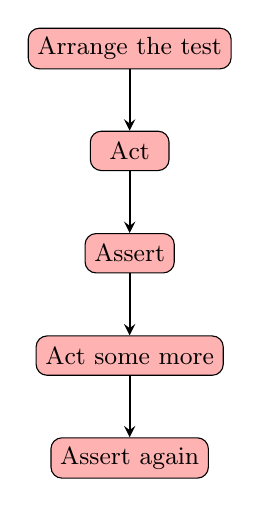
\begin{tikzpicture}[node distance=1.3cm]
            \node (arrange1) [startstop] {\small{Arrange the test}};
            \node (act1) [startstop, below of=arrange1] {\small{Act}};
            \node (assert1) [startstop, below of=act1] {\small{Assert}};
            \node (act2) [startstop, below of=assert1] {\small{Act some more}};
            \node (assert2) [startstop, below of=act2] {\small{Assert again}};
            \draw [arrow] (arrange1) -- (act1);
            \draw [arrow] (act1) -- (assert1);
            \draw [arrow] (assert1) -- (act2);
            \draw [arrow] (act2) -- (assert2);
          \end{tikzpicture}
        \end{center}
      \end{minipage}
    \end{column}
    \begin{column}[]{0.5\textwidth}
      \begin{itemize}
        \item Avoid multiple arrange, act, and assert sections.
      \end{itemize}
    \end{column}
  \end{columns}
\end{frame}

% Having if statements is also an anti-pattern. If you have if statements in the
% act section, if indicates the test is verifies too many things at once.
% The code listing on the left also demonstrates why if statements should be
% avoided in tests. Turns out, cap.records has only 4 elements, i == 4 never
% got verified.
\begin{frame}{Things to avoid for unit tests}
  \begin{columns}[T]
    \begin{column}[]{0.5\textwidth}
      \begin{minipage}{\linewidth}
        \avoidifpkd
      \end{minipage}
    \end{column}
    \begin{column}[]{0.5\textwidth}
      \begin{itemize}
        \item Avoid multiple arrange, act, and assert sections.
        \item Avoid \texttt{if} statements. 
      \end{itemize}
    \end{column}
  \end{columns}
\end{frame}

% Hurts readability, why is there valid and invalid next to each other?
% What if we refactor is_delivery_valid(), do we need to rename all the tests?
% Additional cognitive load to figure out what behavior this test is testing.
\begin{frame}{Naming a unit test}
  \begin{columns}[T]
    \begin{column}[]{0.55\textwidth}
      \begin{minipage}{\linewidth}
        \rigidname
      \end{minipage}
    \end{column}
    \begin{column}[]{0.45\textwidth}
      \begin{itemize}
        \item A rigid convention such as \texttt{<method>\_<scenario>\_<expected>}
        isn't as helpful as plain English
      \end{itemize}
    \end{column}
  \end{columns}
\end{frame}

\begin{frame}{Naming a unit test}
  \begin{columns}[T]
    \begin{column}[]{0.55\textwidth}
      \begin{minipage}{\linewidth}
        \rigidname
        \verbosename
      \end{minipage}
    \end{column}
    \begin{column}[]{0.45\textwidth}
      \begin{itemize}
        \item A rigid convention such as \texttt{<method>\_<scenario>\_<expected>}
        isn't as helpful as plain English
        \item Should not be too verbose
      \end{itemize}
    \end{column}
  \end{columns}
\end{frame}

% "considered" can be removed without losing meaning. "should be" makes this sound
% like a wish, can be replaced with "is" to represent that this is a fact about
% the software we're developing. There is not need to avoid basic English grammar,
% adding the article "a" helps this read like a normal sentence.
\begin{frame}{Naming a unit test}
  \begin{columns}[T]
    \begin{column}[]{0.55\textwidth}
      \begin{minipage}{\linewidth}
        \rigidname
        \verbosename
        \concisename
      \end{minipage}
    \end{column}
    \begin{column}[]{0.45\textwidth}
      \begin{itemize}
        \item A rigid convention such as \texttt{<method>\_<scenario>\_<expected>}
        isn't as helpful as plain English
        \item Should not be too verbose
      \end{itemize}
    \end{column}
  \end{columns}
\end{frame}

\begin{frame}{Parametrizing tests}
  \footnotesize{\textit{Parametrization, also spelled parameterization, parametrisation
  or parameterisation, is the process of defining or choosing parameters.} --- Wikipedia}
  \begin{columns}[T]
    \begin{column}[]{0.5\textwidth}
      \begin{minipage}{\linewidth}
        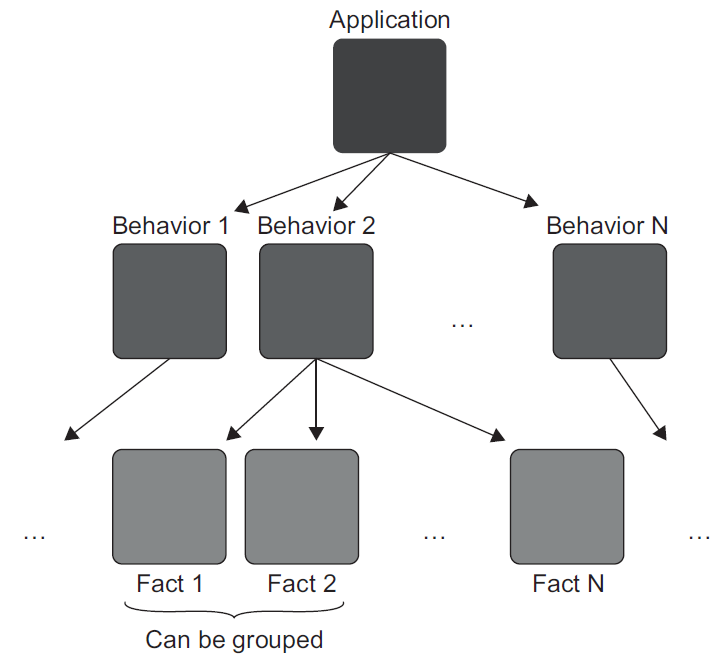
\includegraphics[width=\textwidth]{images/parametrized_tests.png}
      \end{minipage}
    \end{column}
    \begin{column}[]{0.5\textwidth}
      \begin{itemize}
        \item The number of tests can become unmanageable if each component/behavior
        of the application is tested with its own test.
        \item Some (similar) behaviors can be grouped into a single test using
        parametrization.
      \end{itemize}
    \end{column}
  \end{columns}
\end{frame}

\begin{frame}{Parametrizing tests}
  \begin{minipage}{\textwidth}
    Behavior: The soonest allowed delivery date is two days from now. 
  \end{minipage}
  \vfill
  \begin{minipage}{\textwidth}
    In addition to \texttt{test\_delivery\_with\_a\_past\_date\_is\_invalid}, we
    need to add three more:

    \additionalbehavior

    This would result in four test methods, with the only difference between them
    being the delivery date.
  \end{minipage}
\end{frame}

% This comes at a cost, it's now hard to figure out what facts the test method
% represent.
\begin{frame}{Parametrizing tests}
  \begin{minipage}{\textwidth}
    Behavior: The soonest allowed delivery date is two days from now. 
  \end{minipage}
  \begin{columns}[T]
    \begin{column}{0.5\textwidth}
      \begin{minipage}{\textwidth}
        \parametrizeall
      \end{minipage}
    \end{column}
    \begin{column}{0.5\textwidth}
      \begin{itemize}
        \item Significantly reduce the amount of test code
      \end{itemize}
    \end{column}
  \end{columns}
\end{frame}

\begin{frame}{Parametrizing tests (meaningfully)}
  \begin{minipage}{\textwidth}
    Behavior: The soonest allowed delivery date is two days from now. 
  \end{minipage}
  \begin{columns}[T]
    \begin{column}{0.5\textwidth}
      \begin{minipage}{\textwidth}
        \parametrizesome
      \end{minipage}
    \end{column}
    \begin{column}{0.5\textwidth}
      \begin{itemize}
        \item Significantly reduce the amount of test code
        \item Do not ``over parametrize'' if the scenarios are complicated
      \end{itemize}
    \end{column}
  \end{columns}
\end{frame}

\begin{frame}{Using an assertion library (optional)}
  \begin{minipage}{\textwidth}
    An assertion library like \texttt{assertpy} can improve test readability by
    making the assert section read like plain English.
  \end{minipage}
  \begin{columns}[T]
    \begin{column}{0.5\textwidth}
      \begin{minipage}{\textwidth}
        \assertionlibrary
      \end{minipage}
    \end{column}
    \begin{column}{0.5\textwidth}
      \begin{itemize}
        \item Introduces additional dependencies
      \end{itemize}
    \end{column}
  \end{columns}
\end{frame}

\begin{frame}{Using an assertion library (optional)}
  \begin{minipage}{\textwidth}
    An assertion library like \texttt{assertpy} can improve test readability by
    making the assert section read like plain English.
  \end{minipage}
  \begin{columns}[T]
    \begin{column}{0.5\textwidth}
      \begin{minipage}{\textwidth}
        \assertionlibrary

        Bonus: \texttt{Chai} assertion library
        \chailibrary
      \end{minipage}
    \end{column}
    \begin{column}{0.5\textwidth}
      \begin{itemize}
        \item Introduces additional dependencies
      \end{itemize}
    \end{column}
  \end{columns}
\end{frame}

% There are three things to take into account for evaluating how well a test
% protects against regression.
\begin{frame}{Recognizing a good unit test}
  \focus{The four pillars of a good unit test}
  \begin{itemize}
    \item Protection against regression
    \begin{itemize}
      \item Amount of code executed during the test
      \item Complexity of that code
      \item The code's domain significance
    \end{itemize}
    \item Resistance against refactoring
    \item Fast feedback
    \begin{itemize}
      \item "Fast enough"
      \item Can be run more often to detect regressions
    \end{itemize}
    \item Maintainability
    \begin{itemize}
      \item How hard is it to understand the test: Test code quality matters as
      much as production code
      \item How hard is it to run the test
    \end{itemize}
  \end{itemize}
\end{frame}

\begin{frame}{The second pillar: Resistance to refactoring}
  \begin{minipage}{\linewidth}
    \textit{Refactoring} means changing existing code without modifying its
    observable behavior.
  \end{minipage}
  \vfill
  \hideit{
    \begin{minipage}{\linewidth}
      \focus{Scenario:} You developed a new feature and everything works great. The
      feature is working as intended and all the tests are passing.

      \medskip
      
      You decide to clean up the code before submitting the PR. Some refactoring here
      and there, and the code ends up looking better than before.

      \medskip
      
      Except one thing --- the tests are failing. But the feature is still working
      perfectly, just as before. Turns out the tests are written in such a way that
      they fail with any modifications to the underlying code.

      \medskip

      This situation is a \textit{false positive}.
    \end{minipage}
    \vfill
    \begin{minipage}{\linewidth}
      Why is this so important that it deserves its own slide?

      \begin{itemize}
        \item Enable sustainable project growth
        \item Provide early warning to regressions
        \item Give confidence that code changes won't lead to regressions
      \end{itemize}
    \end{minipage}
  }
\end{frame}

\begin{frame}{The second pillar: Resistance to refactoring}
  \begin{minipage}{\linewidth}
    \textit{Refactoring} means changing existing code without modifying its
    observable behavior.
  \end{minipage}
  \vfill
  \begin{minipage}{\linewidth}
    \focus{Scenario:} You developed a new feature and everything works great. The
    feature is working as intended and all the tests are passing.

    \medskip
    
    You decide to clean up the code before submitting the PR. Some refactoring here
    and there, and the code ends up looking better than before.

    \medskip
    
    Except one thing --- the tests are failing. But the feature is still working
    perfectly, just as before. Turns out the tests are written in such a way that
    they fail with any modifications to the underlying code.

    \medskip

    This situation is a \textit{false positive}.
  \end{minipage}
  \vfill
  \hideit{
    \begin{minipage}{\linewidth}
      Why is this so important that it deserves its own slide?

      \begin{itemize}
        \item Enable sustainable project growth
        \item Provide early warning to regressions
        \item Give confidence that code changes won't lead to regressions
      \end{itemize}
    \end{minipage}
  }
\end{frame}

% False positives interfere with these benefits as you no longer perceive it as a
% reliable safety net. This may lead to fewer refactoring or more additional
% manual testing even when the tests pass.
\begin{frame}{The second pillar: Resistance to refactoring}
  \begin{minipage}{\linewidth}
    \textit{Refactoring} means changing existing code without modifying its
    observable behavior.
  \end{minipage}
  \vfill
  \begin{minipage}{\linewidth}
    \focus{Scenario:} You developed a new feature and everything works great. The
    feature is working as intended and all the tests are passing.

    \medskip
    
    You decide to clean up the code before submitting the PR. Some refactoring here
    and there, and the code ends up looking better than before.

    \medskip
    
    Except one thing --- the tests are failing. But the feature is still working
    perfectly, just as before. Turns out the tests are written in such a way that
    they fail with any modifications to the underlying code.

    \medskip

    This situation is a \textit{false positive}.
  \end{minipage}
  \vfill
  \begin{minipage}{\linewidth}
    Why is this so important that it deserves its own slide?

    \begin{itemize}
      \item Enable sustainable project growth
      \item Provide early warning to regressions
      \item Give confidence that code changes won't lead to regressions
    \end{itemize}
  \end{minipage}
\end{frame}

\begin{frame}{How to avoid false positives?}
  Number of false positives is directly related to how the test is structured.
  \begin{itemize}
    \item The more the test is coupled to the implementation detail, the more false
    positives it generates.
  \end{itemize}

  \focus{Solution:} Verify the end result (observable behavior) the SUT delivers,
  not the steps it takes to do that. The best way is to structure the test to tell
  a story about the problem domain.
\end{frame}

\begin{frame}{Example: Testing MessageRenderer}
  \rendererimpl
\end{frame}

\begin{frame}{Example: Testing MessageRenderer}
  \renderertestone
\end{frame}

\begin{frame}{Example: Testing MessageRenderer}
  \renderertestone

  Does this really verify \texttt{MessageRenderer}'s observable behavior?
  \begin{itemize}
    \item What if you rearrange the sub-renderers?
    \item What if you replace one of the sub-renderers?
    \item What if you stop using sub-renderers and implement the rendering directly?
  \end{itemize}
  Does this affect the rendered HTML document? Does the test fail?
\end{frame}

\begin{frame}{Example: Testing MessageRenderer}
  \renderertesttwo

  This test treats \texttt{MessageRenderer} as a black box and is only interested
  in its observable behavior.
  \begin{center}
    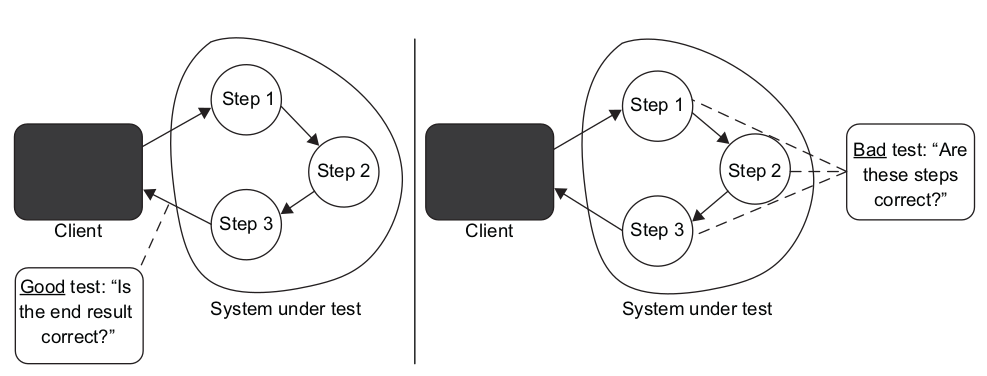
\includegraphics[width=0.8\textwidth]{images/observable_behavior_vs_implementation.png}
  \end{center}
\end{frame}

% The relationship between the first and second pillar can be visualized in this
% confusion matrix. "Functionality is" is the GT and "Test result" is the prediction.
\begin{frame}{Dynamics between the first and second pillar}
  \begin{columns}[T]
    \begin{column}[]{0.55\textwidth}
      \begin{minipage}{\linewidth}
        \begingroup
        \def\arraystretch{1.25}
        \begin{tabular}{|l|l|l|l|}
          \hline
          \multicolumn{2}{|l|}{\multirow{2}{*}{}} & \multicolumn{2}{l|}{Functionality is} \\
          \cline{3-4}
          \multicolumn{1}{|l}{} & & Correct & Broken \\
          \hline
          \multirow{2}{*}[-0.7em]{\begin{tabular}{@{}l@{}}Test \\ result \end{tabular}} & Passes
            & \cellcolor{lime}\begin{tabular}{@{}l@{}} Correct \\ inference \\ (TN) \end{tabular}
            & \cellcolor{pink}\begin{tabular}{@{}l@{}} Type II \\ error \\ (FN) \end{tabular}\tikzmark{a} \\
          \cline{2-4}
          & Fails
            & \cellcolor{pink}\begin{tabular}{@{}l@{}} Type I \\ error \\ (FP)\tikzmark{b} \end{tabular}
            & \cellcolor{lime}\begin{tabular}{@{}l@{}} Correct \\ inference \\ (TP) \end{tabular} \\
          \hline
        \end{tabular}
        \begin{tikzpicture}[remember picture, overlay]
          \node [right=1.6cm,above=0.25cm,minimum width=0pt,text width=1.5cm] at ({pic cs:a}) (A) {Protection against regression};
          \node [right=1.6cm,below=0.25cm,minimum width=0pt,text width=2cm] at ({pic cs:b}) (B) {Resistance to refactoring};
          \draw [<-,out=5,in=270] ([xshift=15pt]{pic cs:a}) to (A);
          \draw [<-,out=270,in=180] ([xshift=15pt]{pic cs:b}) to (B);
        \end{tikzpicture}
        \endgroup
      \end{minipage}
    \end{column}
    \begin{column}[]{0.45\textwidth}
    \end{column}
  \end{columns}
\end{frame}

% In the short term, FPs are not as bad as FN. The importance of refactoring is
% not immediate, it increases gradually over time. Most people tend to focus
% solely on improving the first pillar but this is not enough to build a valuable
% test suite which helps sustain project growth.
\begin{frame}{Dynamics between the first and second pillar}
  \begin{columns}[T]
    \begin{column}[]{0.55\textwidth}
      \begin{minipage}{\linewidth}
        \begingroup
        \def\arraystretch{1.25}
        \begin{tabular}{|l|l|l|l|}
          \hline
          \multicolumn{2}{|l|}{\multirow{2}{*}{}} & \multicolumn{2}{l|}{Functionality is} \\
          \cline{3-4}
          \multicolumn{1}{|l}{} & & Correct & Broken \\
          \hline
          \multirow{2}{*}[-0.7em]{\begin{tabular}{@{}l@{}}Test \\ result \end{tabular}} & Passes
            & \cellcolor{lime}\begin{tabular}{@{}l@{}} Correct \\ inference \\ (TN) \end{tabular}
            & \cellcolor{pink}\begin{tabular}{@{}l@{}} Type II \\ error \\ (FN) \end{tabular}\tikzmark{a} \\
          \cline{2-4}
          & Fails
            & \cellcolor{pink}\begin{tabular}{@{}l@{}} Type I \\ error \\ (FP)\tikzmark{b} \end{tabular}
            & \cellcolor{lime}\begin{tabular}{@{}l@{}} Correct \\ inference \\ (TP) \end{tabular} \\
          \hline
        \end{tabular}
        \begin{tikzpicture}[remember picture, overlay]
          \node [right=1.6cm,above=0.25cm,minimum width=0pt,text width=1.5cm] at ({pic cs:a}) (A) {Protection against regression};
          \node [right=1.6cm,below=0.25cm,minimum width=0pt,text width=2cm] at ({pic cs:b}) (B) {Resistance to refactoring};
          \draw [<-,out=5,in=270] ([xshift=15pt]{pic cs:a}) to (A);
          \draw [<-,out=270,in=180] ([xshift=15pt]{pic cs:b}) to (B);
        \end{tikzpicture}
        \endgroup
      \end{minipage}
    \end{column}
    \begin{column}[]{0.45\textwidth}
      \begin{itemize}
        \item How good the test is at indicating the \focus{presence} of bugs: Protection against regression
        \item How good the test is at indicating the \focus{absence} of bugs: Resistance of refactoring
      \end{itemize}
      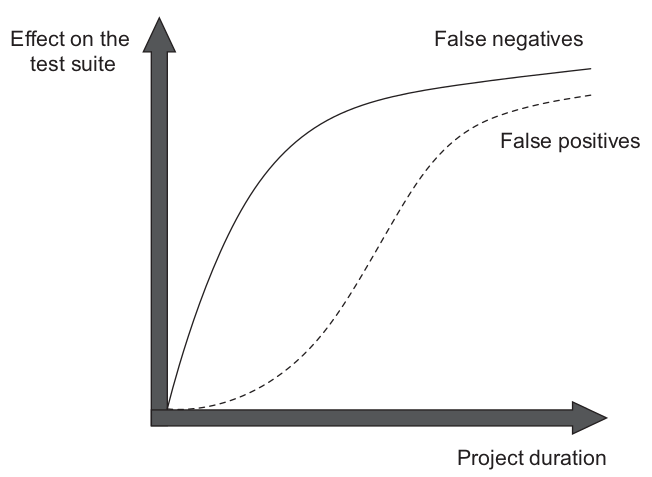
\includegraphics[width=\textwidth]{images/test_suite_fnfp.png}
    \end{column}
  \end{columns}
\end{frame}

% The first three pillars are mutually exclusive, you have to sacrifice one to
% maximize the remaining two. Because of the multiplication principle in estimating
% a test's value, you can't just forgo one of the attributes to focus on the
% others.
\begin{frame}{In search of an ideal test}
  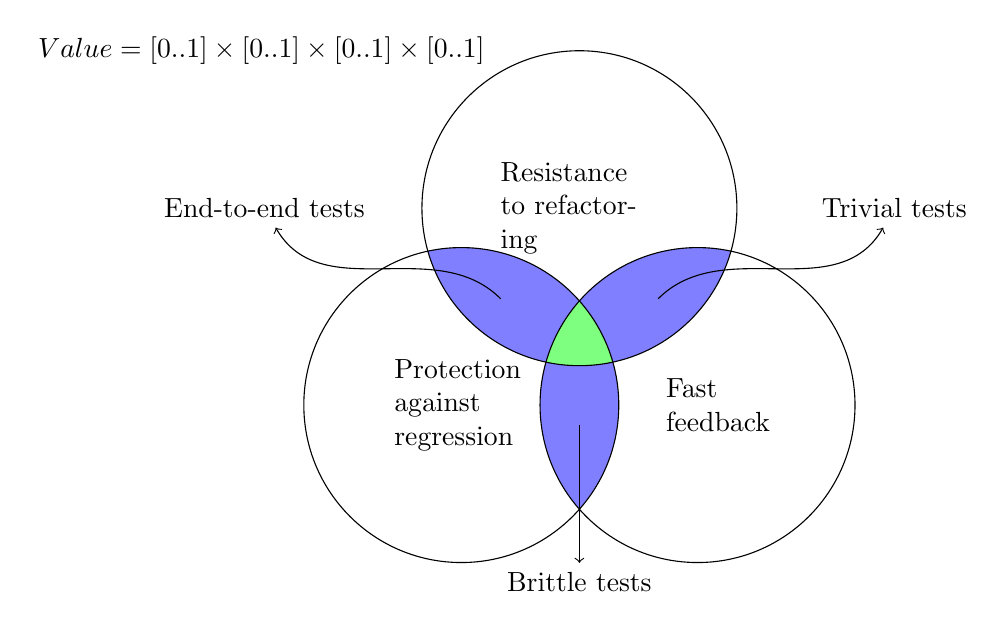
\begin{tikzpicture}
    \begin{scope}[fill opacity=0.5]
      \clip (0, 0) circle (2);
      \fill[blue] (-1.5, -2.5) circle (2);
    \end{scope}
    \begin{scope}[fill opacity=0.5]
      \clip (-1.5, -2.5) circle (2);
      \fill[blue] (1.5, -2.5) circle (2);
    \end{scope}
    \begin{scope}[fill opacity=0.5]
      \clip (1.5, -2.5) circle (2);
      \fill[blue] (0, 0) circle (2);
    \end{scope}
    \begin{scope}
      \clip (0, 0) circle (2);
      \clip (1.5, -2.5) circle (2);
      \fill[white] (-1.5, -2.5) circle (2);
    \end{scope}
    \begin{scope}[fill opacity=0.5]
      \clip (0, 0) circle (2);
      \clip (1.5, -2.5) circle (2);
      \fill[green] (-1.5, -2.5) circle (2);
    \end{scope}
    \draw (-7, 2) node [text=black,right] {$Value = [0..1] \times [0..1] \times [0..1] \times [0..1]$};
    \draw (0, 0) circle (2);
    \draw (-1.5, -2.5) circle (2);
    \draw (1.5, -2.5) circle (2);
    \draw (0, 0) node [text=black, text width=2cm] {Resistance to refactoring};
    \draw (-1.5, -2.5) node [text=black, text width=1.7cm] {Protection against regression};
    \draw (1.5, -2.5) node [xshift=1em,text=black, text width=1.5cm] {Fast\\feedback};
    \node at (-4, 0) (label A) {End-to-end tests};
    \node at (4, 0) (label B) {Trivial tests};
    \node at (0, -4.75) (label C) {Brittle tests};
    \coordinate (A) at (-1, -1.15);
    \coordinate (B) at (1, -1.15);
    \coordinate (C) at (0, -2.75);
    \draw [<-,out=300] (label A) to (A);
    \draw [<-,in=45,out=240] (label B) to (B);
    \draw [<-] (label C) to (C);
  \end{tikzpicture} 
\end{frame}

\begin{frame}{In search of an ideal test}
  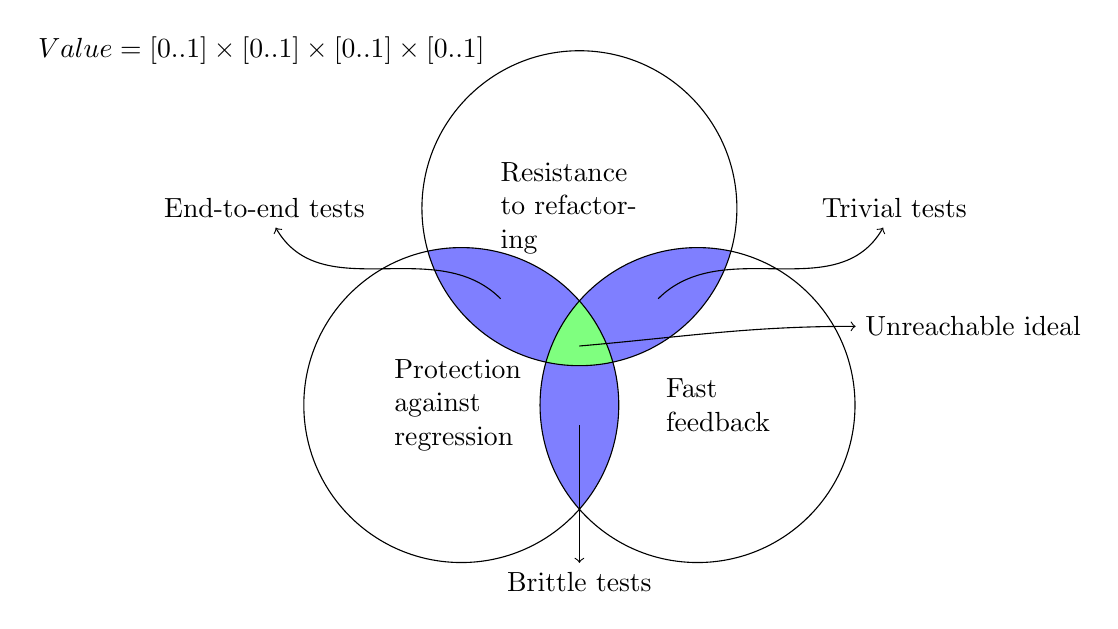
\begin{tikzpicture}
    \begin{scope}[fill opacity=0.5]
      \clip (0, 0) circle (2);
      \fill[blue] (-1.5, -2.5) circle (2);
    \end{scope}
    \begin{scope}[fill opacity=0.5]
      \clip (-1.5, -2.5) circle (2);
      \fill[blue] (1.5, -2.5) circle (2);
    \end{scope}
    \begin{scope}[fill opacity=0.5]
      \clip (1.5, -2.5) circle (2);
      \fill[blue] (0, 0) circle (2);
    \end{scope}
    \begin{scope}
      \clip (0, 0) circle (2);
      \clip (1.5, -2.5) circle (2);
      \fill[white] (-1.5, -2.5) circle (2);
    \end{scope}
    \begin{scope}[fill opacity=0.5]
      \clip (0, 0) circle (2);
      \clip (1.5, -2.5) circle (2);
      \fill[green] (-1.5, -2.5) circle (2);
    \end{scope}
    \draw (-7, 2) node [text=black,right] {$Value = [0..1] \times [0..1] \times [0..1] \times [0..1]$};
    \draw (0, 0) circle (2);
    \draw (-1.5, -2.5) circle (2);
    \draw (1.5, -2.5) circle (2);
    \draw (0, 0) node [text=black, text width=2cm] {Resistance to refactoring};
    \draw (-1.5, -2.5) node [text=black, text width=1.7cm] {Protection against regression};
    \draw (1.5, -2.5) node [xshift=1em,text=black, text width=1.5cm] {Fast\\feedback};
    \node at (-4, 0) (label A) {End-to-end tests};
    \node at (4, 0) (label B) {Trivial tests};
    \node at (0, -4.75) (label C) {Brittle tests};
    \node at (5, -1.5) (label D) {Unreachable ideal};
    \coordinate (A) at (-1, -1.15);
    \coordinate (B) at (1, -1.15);
    \coordinate (C) at (0, -2.75);
    \coordinate (D) at (0, -1.75);
    \draw [<-,out=300] (label A) to (A);
    \draw [<-,in=45,out=240] (label B) to (B);
    \draw [<-] (label C) to (C);
    \draw [<-,in=5,out=180] (label D) to (D);
  \end{tikzpicture} 
\end{frame}

% Black-box testing examines the functionality of a system without knowing its
% internal structure, typically built around specs and requirements.
% White-box testing verifies the application's inner workings, tests are derived
% from the source code.
% Prefer black-box testing over white-box testing by default to maximize
% resistance to refactoring. But white-box method can still be used when
% analyzing the tests, use code coverage tools to see which code branches are not
% exercised and then test them as if you don't know the inner workings.
\begin{frame}{In search of an ideal test}
  \begin{columns}[T]
    \begin{column}[]{0.55\textwidth}
      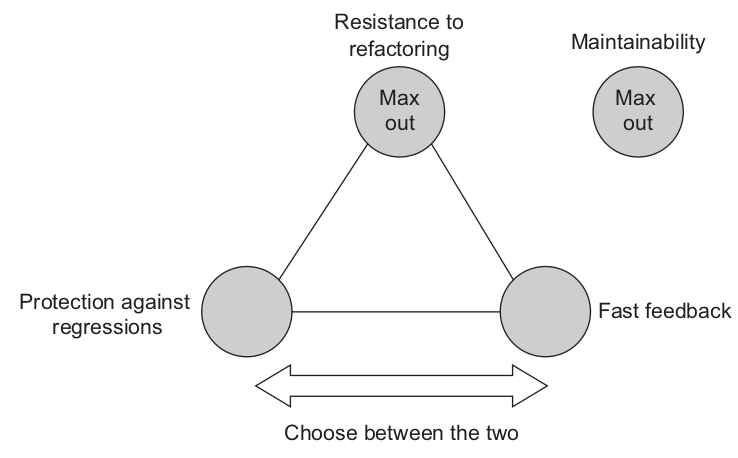
\includegraphics[width=\textwidth]{images/ideal_strategy.png}
    \end{column}
    \begin{column}[]{0.45\textwidth}
      \begin{itemize}
        \item \textit{Resistance to refactoring} is non-negotiable: Almost a binary choice
        \item Test automation concepts can be traced back to the four pillars:
        \begin{itemize}
          \item The Test Pyramid
          \item White-box versus black-box testing
        \end{itemize}
      \end{itemize}
    \end{column}
  \end{columns}
\end{frame}

\section{Mocks and test fragility}
\begin{frame}{Differentiating mocks from stubs}
  \begin{columns}[T]
    \begin{column}[]{0.5\textwidth}
      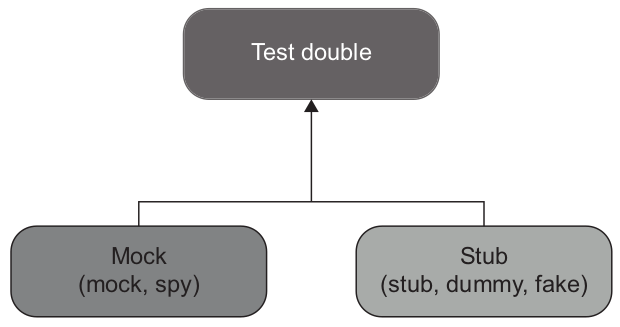
\includegraphics[width=0.85\textwidth]{images/test_doubles.png}
    \end{column}
    \begin{column}[]{0.5\textwidth}
      \begin{itemize}
        \item Test doubles can be grouped into two types: \focus{mocks} and \focus{stubs}
      \end{itemize}
    \end{column}
  \end{columns}
\end{frame}

\begin{frame}{Differentiating mocks from stubs}
  \begin{columns}[T]
    \begin{column}[]{0.5\textwidth}
      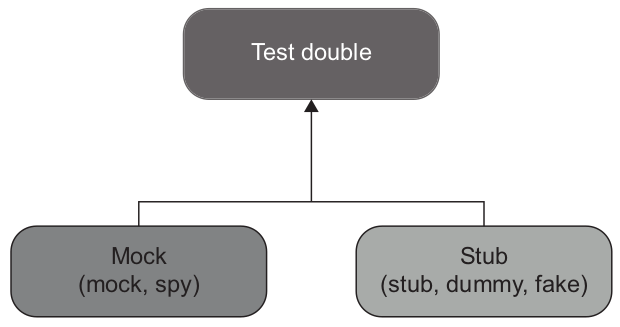
\includegraphics[width=0.85\textwidth]{images/test_doubles.png}
      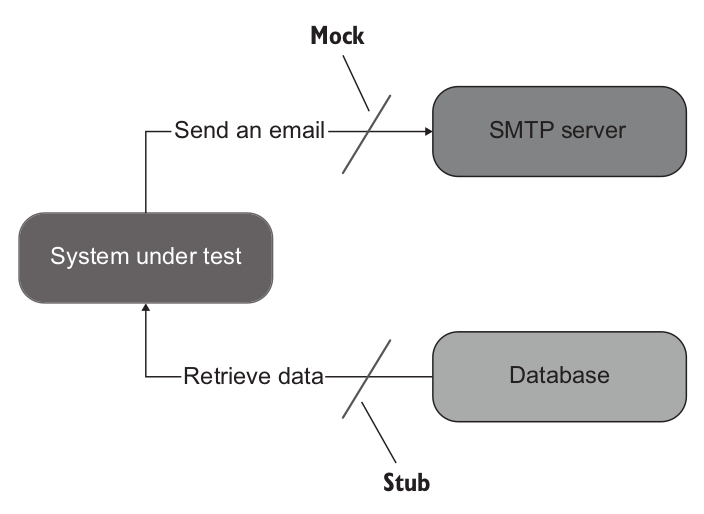
\includegraphics[width=0.85\textwidth]{images/stub_vs_mock.png}
    \end{column}
    \begin{column}[]{0.5\textwidth}
      \begin{itemize}
        \item Test doubles can be grouped into two types: \focus{mocks} and \focus{stubs}
        \item \focus{Mocks} emulate and examine \textit{outcoming} interactions
        \item \focus{Stubs} emulate \textit{incoming} interactions
      \end{itemize}
    \end{column}
  \end{columns}
\end{frame}
\end{document}
